\documentclass[lecture.tex]{subfiles}

\begin{document}

\exercice{}
%\video{https://youtu.be/blablabla}
\enonce{rdm-0011}{Section L}


\begin{center}
  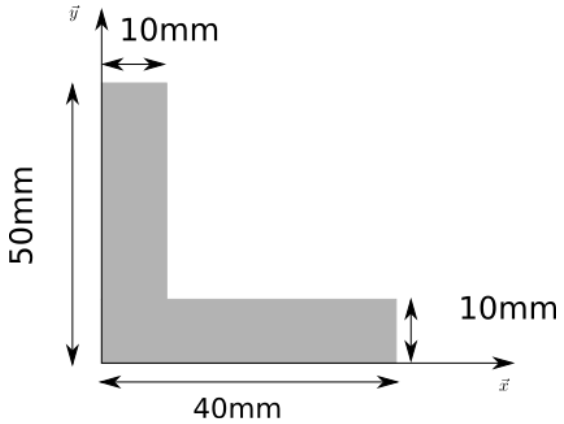
\includegraphics[scale=0.3]{exo-moment-quadratique-section-L.png}
\end{center}

\begin{enumerate}
  \item Trouver les coordonnées du centre de gravité de la section
  \item Calculer les moments quadratiques $I_x$, $I_y$ par rapport aux axes $\vec{x}$ et $\vec{y}$
  \item Calculer $I_{xG}$, $I_{yG}$ par rapport au repère barycentrique.
  \item Trouver $I_{xy}(G)$
\end{enumerate}

\finenonce{rdm-0011}
\finexercice



\end{document}
